\documentclass[addpoints,12pt, answers]{exam}

\usepackage{amsmath, amsthm, amssymb, amsfonts}
\usepackage{thmtools}
\usepackage{graphicx}
\usepackage[hidelinks]{hyperref}
\usepackage[utf8]{inputenc}
\usepackage[english]{babel}
\usepackage{framed}
\usepackage[dvipsnames]{xcolor}
\usepackage{tcolorbox}
\usepackage{tabto}
\usepackage{titling}
\usepackage{tikz}

\usepackage{changepage} % for the adjustwidth environment


\colorlet{LightGray}{White!90!Periwinkle}
\colorlet{LightOrange}{Orange!15}
\colorlet{LightGreen}{Green!15}

\newcommand{\HRule}[1]{\rule{\linewidth}{#1}}

\declaretheoremstyle[name=Theorem,]{thmsty}
\declaretheorem[style=thmsty,numberwithin=section]{theorem}
\tcolorboxenvironment{theorem}{colback=LightGray}

\declaretheoremstyle[name=Proposition,]{prosty}
\declaretheorem[style=prosty,numberlike=theorem]{proposition}
\tcolorboxenvironment{proposition}{colback=LightOrange}

\declaretheoremstyle[name=Principle,]{prcpsty}
\declaretheorem[style=prcpsty,numberlike=theorem]{principle}
\tcolorboxenvironment{principle}{colback=LightGreen}

%% This latex package provides all the utilities for
%% 15150 assignments development.
%% This package is intended to be included in writeup.tex at
%% problem level.
%% For a full list of custom commands, check 15150toolbox.md
%%
%% @author: Jolin Zhou
%% @email: jiulingz@andrew.cmu.edu

\NeedsTeXFormat{LaTeX2e}
\ProvidesPackage{toolbox-reduced}[2020/05/15 Latex toolbox for M20 Lecture Notes]

%%%%%%%%%%%%%%%%%%%%%
%% Robust Commands %%
%%%%%%%%%%%%%%%%%%%%%
% used throughout this package
\RequirePackage{etoolbox}
\RequirePackage{xparse}

% hyperlink/reference
\RequirePackage{xcolor}

% graphics
\RequirePackage{graphicx}

% emphasize
\usepackage{bm}
\DeclareTextFontCommand{\emph}{\bfseries\em}

%%%%%%%%%%%%%%%%%%%%%%%%%%%%%%%
%% Task related environments %%
%%%%%%%%%%%%%%%%%%%%%%%%%%%%%%%
% environment colors
\RequirePackage{xcolor}
\definecolor{task_color}      {RGB}{ 64, 100, 255}
\definecolor{solution_color}  {RGB}{  0,   0, 128}
\definecolor{constraint_color}{RGB}{175,   0,   0}

% task environment
\RequirePackage{framed}
\providerobustcmd{\attribute}[1]{}
\newcounter{taskcounter}
\NewDocumentEnvironment{task}{m}
{
  \stepcounter{taskcounter}
  \textbf{Task \arabic{taskcounter}.}\attribute{#1}
  \phantomsection
  \addcontentsline{toc}{subsubsection}{\textcolor{task_color}{\textbf{Task \arabic{taskcounter}.}\texorpdfstring{\attribute{#1}}{}}}
  \par
}
{
  \ifdef{\loadsolution}
    {{
      \color{solution_color}
      \begin{framed}
        \textbf{Solution \arabic{taskcounter}.}\par
        \loadsolution{#1}
      \end{framed}
    }}
    {}
  \vspace{1em}
}

% constraint environment
\newenvironment{constraint}{\color{constraint_color}\textbf{Constraint:}}{}

%%%%%%%%%%%%%%%%%%%%%%%%
%% Code Specification %%
%%%%%%%%%%%%%%%%%%%%%%%%
% spec
\RequirePackage{framed}
\usepackage{mdframed}
\newrobustcmd{\spec}[4]{
\begin{mdframed}
\code{#1 : #2}\par
\ifstrempty{#3}{}{\par REQUIRES: #3}
\ifstrempty{#4}{}{\par ENSURES: #4}
\end{mdframed}
}

%%%%%%%%%%%%%%%%%%%%%
%% Text Formatting %%
%%%%%%%%%%%%%%%%%%%%%
% symbols
\RequirePackage{amssymb, amsmath, amsthm, amsfonts}

\newrobustcmd{\stepsTo}{\Longrightarrow}
\newrobustcmd{\stepsToStar}{\Longrightarrow}
\newrobustcmd{\stepsToIn}[1]{\Longrightarrow^{#1}}

\newrobustcmd{\eeq}{\cong}

%%%%%%%%%%%%%%%%%%%%%%
%% Code Environment %%
%%%%%%%%%%%%%%%%%%%%%%
% code style
\RequirePackage{listings}
\RequirePackage{lstautogobble}
\RequirePackage{xcolor}

\newlength{\MaxSizeOfLineNumbers}%
\settowidth{\MaxSizeOfLineNumbers}{99}% Adjust to maximum number of lines
\addtolength{\MaxSizeOfLineNumbers}{.5ex}%

\newcommand{\darkBg}{8b98ad}
\definecolor{background_color}{RGB}{225, 225, 225}
\definecolor{string_color}    {RGB}{180, 156,   0}
\definecolor{keyword_color}   {RGB}{ 64, 100, 255}
\definecolor{comment_color}   {RGB}{  140, 140, 140}
\definecolor{number_color}    {RGB}{ 84,  84,  84}
\lstdefinestyle{15150code}{
    basicstyle=\ttfamily,
    numberstyle=\tiny\ttfamily\color{number_color},
    stringstyle=\color{string_color},
    keywordstyle=\color{blue!90!black},
    commentstyle=\color{comment_color},
    numbers=left,
    rulesepcolor=\color{black!20!white},
    linewidth=\textwidth,
    columns=fixed,
    tabsize=2,
    xleftmargin=\MaxSizeOfLineNumbers,
    breaklines=true,
    keepspaces=true,
    showstringspaces=false,
    captionpos=b,
    autogobble=true,
    mathescape=true,
    literate={~}{{$\thicksim$}}1
             {~=}{{$\eeq$}}1
}
\lstdefinelanguage{sml}{
    language=ML,
    morestring=[b]",
    morecomment=[s]{(*}{*)},
    morekeywords={
        bool, char, exn, int, real, string, unit, list, option,
        EQUAL, GREATER, LESS, NONE, SOME, nil,
        andalso, orelse, true, false, not,
        if, then, else, case, of, as,
        let, in, end, local, val, rec,
        datatype, type, exception, handle,
        fun, fn, op, raise, ref,
        structure, struct, signature, sig, functor,
        include, open, use, infix, infixr, o, print
    }
}

\usepackage[T1]{fontenc}

\makeatletter
\newenvironment{btHighlight}[1][]
{\begingroup\tikzset{bt@Highlight@par/.style={#1}}\begin{lrbox}{\@tempboxa}}
{\end{lrbox}\bt@HL@box[bt@Highlight@par]{\@tempboxa}\endgroup}

\newcommand\btHL[1][]{%
  \begin{btHighlight}[#1]\bgroup\aftergroup\bt@HL@endenv%
}
\def\bt@HL@endenv{%
  \end{btHighlight}%
  \egroup
}
\newcommand{\bt@HL@box}[2][]{%
  \tikz[#1]{%
    \pgfpathrectangle{\pgfpoint{1pt}{0pt}}{\pgfpoint{\wd #2}{\ht #2}}%
    \pgfusepath{use as bounding box}%
    \node[anchor=base west, fill=yellow!45,outer sep=0pt,inner xsep=1pt, inner ysep=0pt, rounded corners=3pt, minimum height=\ht\strutbox+1pt,#1]{\raisebox{1pt}{\strut}\strut\usebox{#2}};
  }%
}

\newenvironment{atHighlight}[1][]
{\begingroup\tikzset{at@Highlight@par/.style={#1}}\begin{lrbox}{\@tempboxa}}
{\end{lrbox}\at@HL@box[at@Highlight@par]{\@tempboxa}\endgroup}

\newcommand\atHL[1][]{%
  \begin{atHighlight}[#1]\bgroup\aftergroup\at@HL@endenv%
}
\def\at@HL@endenv{%
  \end{atHighlight}%
  \egroup
}
\newcommand{\at@HL@box}[2][]{%
  \tikz[#1]{%
    \pgfpathrectangle{\pgfpoint{1pt}{0pt}}{\pgfpoint{\wd #2}{\ht #2}}%
    \pgfusepath{use as bounding box}%
    \node[anchor=base west, fill=red!45,outer sep=0pt,inner xsep=1pt, inner ysep=0pt, rounded corners=3pt, minimum height=\ht\strutbox+1pt,#1]{\raisebox{1pt}{\strut}\strut\usebox{#2}};
  }%
}
\makeatother

% code inline
\newrobustcmd{\code}[2][]{{\sloppy
\ifmmode
    \text{\lstinline[language=sml,style=15150code,#1]`#2`}
\else
    {\lstinline[language=sml,style=15150code,#1]`#2`}%
\fi}}

% code block
\lstnewenvironment{codeblock}[1][]{\lstset{language=sml,style=15150code,numbers=none,#1,moredelim=**[is][\btHL]{`}{`},moredelim=**[is][\atHL]{&}{&}}}{}

% ------------------------------------------------------------------------------

\usepackage{fancyhdr}
\begin{document}

% Set the page style to "fancy"...
\pagestyle{fancy}
%... then configure it.
\fancyhead{} % clear all header fields
\fancyhead[R]{15-150: Principles of Functional Programming}
\fancyhead[L]{Midterm 1}
\fancyfoot[C]{\thepage} % clear all footer fields

% ------------------------------------------------------------------------------
% Cover Page and ToC
% ------------------------------------------------------------------------------

\setlength{\droptitle}{-8em}   % This is your set screw

\title{ \normalsize \textsc{}
		\HRule{1.5pt} \\
		\large \textbf{
      \uppercase{Midterm 1} \\
      15-150 Principles of Functional Programming M23} \\
    \HRule{1.5pt}
    \date{}
}

\maketitle

\vspace{-3cm}

\hspace{-1cm} Name \rule{5cm}{0.4pt} \, Andrew ID \rule{3cm}{0.4pt} \, House \rule{3.5cm}{0.4pt}

\vspace{5pt}

\begin{itemize}
  \item Write your name, Andrew ID, and House name on this page.
  \item This is an 80 minute examination of 6 parts.
  \item Answers should be short and to the point. Obey question constraints, wherever
  they appear, and write syntactically legal SML programs!
  \item In proofs, use valid reasoning, state clearly the kind of induction you are
  doing, and justify each of your steps.
\end{itemize}
\vspace{\fill}

{\small
\vqword{}
\vpword{Max}
\begin{center}
\gradetable[v][questions]
\end{center}
}

\vspace{\fill}

\begin{center}
  Feel free to use this space to draw a joke or meme about functional programming: \\

  \vspace{10pt}

  \fbox{\rule{6in}{0pt}\rule[-0.5ex]{0pt}{2.5in}}
\end{center}


\newpage

% ------------------------------------------------------------------------------

\section*{Questions}

\begin{questions}

\titledquestion{Types and Values}
\textbf{Types and Values}

For each of the expressions below, write its type and value.

\textbf{If the expression is not well-typed then say so and explain your answer briefly.}

\textbf{If the expression does not evaluate to a value then say so and explain your answer briefly.}

If the value is a function, write out the function as an \texttt{fn} expression.

\begin{parts}

  \part[2]\hfill

  \code{(1 + 2, (true, ["hi"]))}

  \textbf{Type:} \begin{solutionorlines}[2em] \code{int * (bool * int list)} \end{solutionorlines}

  \textbf{Value:} \begin{solutionorlines}[2em] \code{(3, (true, ["hi"]))} \end{solutionorlines}


  \part[2] \hfill

  \code{(fn x => true andalso x) true}

  \textbf{Type:} \begin{solutionorlines}[2em] \code{bool} \end{solutionorlines}

  \textbf{Value:} \begin{solutionorlines}[2em] \code{true} \end{solutionorlines}

  \part[2]\hfill

  \begin{codeblock}
  case 2 of
    1 => (fn x => 1 + x)
  | 2 => (fn y => 2 + y)
  | _ => (fn z => 3 + z)
  \end{codeblock}

  \textbf{Type:} \begin{solutionorlines}[2em] \code{int -> int} \end{solutionorlines}

  \textbf{Value:} \begin{solutionorlines}[2em] \code{fn y => 2 + y} \end{solutionorlines}

  \newpage

  \part[2]\hfill

  \begin{codeblock}
  case 2 of
    1 => (fn x => 1 + x)
  | 2 => (fn y => true andalso y)
  | _ => (fn z => 3 + z)
  \end{codeblock}

  \textbf{Type:} \begin{solutionorlines}[2em] ill-typed, case branches do not agree \end{solutionorlines}

  \textbf{Value:} \begin{solutionorlines}[2em] no value because ill-typed! \end{solutionorlines}

  \part[2]\hfill

  \begin{codeblock}
  let
    fun f (x : int) : int list = x :: f x
    val _ = f 150
  in
    2
  end
  \end{codeblock}

  \textbf{Type:} \begin{solutionorlines}[2em] \code{int} \end{solutionorlines}

  \textbf{Value:} \begin{solutionorlines}[2em] no value, loops forever \end{solutionorlines}

\end{parts}

\newpage

\titledquestion{Evaluation and Equivalence}

\textbf{Evaluation and Equivalence}

For each of the questions below, please mark whether they are "true" or
"false". If your answer is false, please briefly justify why.

\begin{parts}
  \part[2]\hfill

  If, for expressions \code{e1, e2 : t}, we have that \code{e1} $\hookrightarrow$ \code{v}, and
  \code{e2} $\hookrightarrow$ \code{v}, for some value \code{v : t}, then it must be
  true that \code{e1} $\stepsTo^*$ \code{e2}.

  \begin{solutionorlines}[2em] False. Consider \code{1 + 1} and \code{2 + 0}. \end{solutionorlines}

  \part[2]\hfill

  If an expression \code{e : t1 -> t2} is total, then \code{e} is also
  valuable.

  \begin{solutionorlines}[2em] True \end{solutionorlines}

  \part[2]\hfill

  \code{(fn (x, y) => (y, x)) (1, 2 + 3)} $\stepsTo^*$ \code{(2 + 3, 1)}

  \begin{solutionorlines}[2em] False, eager evaluation means \code{2 + 3} is evaluated
  first \end{solutionorlines}

  \part[2]\hfill

  For any expression \code{e : t}, \code{SOME e} is valuable.

  \begin{solutionorlines}[2em] False, \code{e} may not terminate. \end{solutionorlines}

  \part[2]\hfill

  For any value \code{v : t}, \code{SOME v} is valuable.

  \begin{solutionorlines}[2em] True. \end{solutionorlines}

\end{parts}

\newpage
\titledquestion{Binary Search Trees}

\textbf{Binary Search Trees}

Recall the type of \code{tree}s, from lecture:
\begin{codeblock}
  datatype tree = Empty | Node of tree * int * tree
\end{codeblock}

A \textit{binary search tree} is a value of the \code{tree} type, that satisfies the
following definition:

\textbf{Definition.} A value \code{v : t} is called a \textit{binary search tree} if:
\begin{enumerate}
  \item It is \code{Empty}.
  \item It is \code{Node (L, x, R)}, where both \code{L} and \code{R} are binary search trees,
  and \code{x} is greater than or equal to every element in \code{L}, and less than or
  equal to every element in \code{R}.
\end{enumerate}


\begin{parts}
  \part[5]\hfill

  Implement a function \code{isGeqTree} which adheres to the following specification:

  \spec
    {isGeqTree}
    {int * tree -> bool}
    {\code{true}}
    {\code{isGeqTree (x, T)} evaluates to \code{true} iff \code{x} is greater than
    or equal to every element of \code{T}.}

  \begin{solutionorbox}[20em]
    \begin{codeblock}
      fun isGeqTree (n : int, Empty : tree) : bool = true
        | isGeqTree (n, Node (L, x, R)) =
            n >= x andalso isGeqTree (n, L) andalso isGeqTree (n, R)
    \end{codeblock}
  \end{solutionorbox}

  \begin{EnvUplevel}
    Assuming that we have implemented an analogous \code{isLeqTree} function,
    with the following specification:

    \vspace{7pt}
    \begin{adjustwidth}{0em}{0em} % adjust the left margin to 2em
    \spec
      {isLeqTree}
      {int * tree -> bool}
      {\code{true}}
      {\code{isLeqTree (x, T)} evaluates to \code{true} iff \code{x} is less than
      or equal to every element of \code{T}.}
    \end{adjustwidth}

    then we can define our \code{isBST} function with the following specification:

    \vspace{7pt}
    \begin{adjustwidth}{0em}{0em} % adjust the left margin to 2em
    \spec
      {isBST}
      {tree -> bool}
      {\code{true}}
      {\code{isBST T} evaluates to \code{true} iff \code{T} is a binary search tree.}
    \end{adjustwidth}

    % TODO: could give to them?
    \begin{codeblock}
      fun isBST (Empty : tree) : bool = true
        | isBST (Node (L, x, R)) =
            isBST L andalso isBST R
            andalso isLeqTree (x, R) andalso isGeqTree (x, L)
    \end{codeblock}
  \end{EnvUplevel}

  \part[2]\hfill

  Assuming that the work of both \code{isGeqTree} and \code{isLeqTree} are
  $O(n)$ in the number of nodes in the tree, write a recurrence for the \textbf{work}
  of \code{isBST}, in terms of $n$, the number of nodes in the input tree, when given
  a \textbf{balanced} tree. You do not need to give a bound.

  You may assume that \code{isLeqTree} has the same complexity as \code{isGeqTree}.

  \begin{solutionorbox}[20em]
    $W_{\code{isBST}}(0) = c_0$
    $W_{\code{isBST}}(n) = 2W_{\code{isBST}}(\frac{n}{2}) +
    W_{\code{isLeqTree}}(\frac{n}{2}) + W_{\code{isGeqTree}}(\frac{n}{2}) + c_1$

    Solves to $O(n \log n)$.
  \end{solutionorbox}

  \newpage

  \part[5]\hfill

  Solve the recurrence from the previous part to obtain a bound in
  $n$. Show your work! You may combine terms of the same asymptotic complexity
  together to simplify your analysis.

  \begin{solutionorbox}[40em]
    By the Tree Method.

    We note that there are $\log n$ levels, $2^i$ nodes per level, and
    approximately $\frac{n}{2^i}c_1$ work per node at level $i$.

    So we get a summation of $\sum_{i=1}^{\log n}(2^i \cdot \frac{n}{2^i} c_1)$
    which simplifies to $\sum_{i = 1}^{\log n}(nc_1)$, which gives us a bound of
    $O(n \log n)$.
  \end{solutionorbox}
\end{parts}

\newpage
\titledquestion{Binary Search Trees, Better}

\textbf{Binary Search Trees, Better}

That's a pretty silly way to do \code{isBST}. Let's try via a different
method.

Recall the \textit{inorder traversal} of a tree, which looks something like this:

\begin{center}
  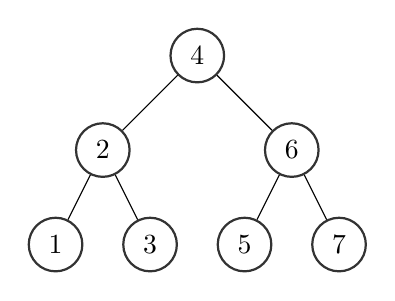
\begin{tikzpicture}
    [level distance=12mm,
    every node/.style={circle,inner sep=4pt, draw=black!80, thick},
    level 1/.style={sibling distance=24mm},
    level 2/.style={sibling distance=12mm},
    ]
    \node {4}
      child {node {2}
        child {node {1}}
        child {node {3}}
      }
      child {node {6}
        child {node {5}}
        child {node {7}}
      };
    \end{tikzpicture}
\end{center}

Essentially, we visit the nodes from "left to right", as a normal
human would read it. It just so happens to be that, if a tree is a binary
search tree, then an inorder traversal of that tree should only visit
nodes in a nondecreasing order.

\begin{parts}

  \part[5]\hfill

  Write a function \code{isNondecreasing}, which satisfies the following
  specification:

  \spec
    {isNondecreasing}
    {int list -> bool}
    {\code{true}}
    {\code{isNondecreasing L} evaluates to \code{true} iff all the elements
    of \code{L} are present in nondecreasing order, from left to right.}

  Test cases:
  \begin{itemize}
    \item \code{isNondecreasing []} $\hookrightarrow$ \code{true}
    \item \code{isNondecreasing [1]} $\hookrightarrow$ \code{true}
    \item \code{isNondecreasing [1, 2, 2, 3]} $\hookrightarrow$ \code{true}
    \item \code{isNondecreasing [1, 3, 2, 4]} $\hookrightarrow$ \code{false}
  \end{itemize}

  \begin{constraint}
    You must implement \code{isNondecreasing} via direct recursion, with
    no helper functions.

    \code{isNondecreasing} must be implemented in $O(n)$ in the length
    of the input list.
  \end{constraint}

  \begin{solutionorbox}[12em]
    \begin{codeblock}
      fun isNondecreasing ([] : int list) = true
        | isNondecreasing [x] = true
        | isNondecreasing (x::y::ys) =
            x <= y andalso isNondecreasing (y::ys)
    \end{codeblock}
  \end{solutionorbox}

  \begin{EnvUplevel}
    With the \code{isNondecreasing} function, we can simply define
    \code{isBST} as follows:

    \begin{codeblock}
      fun isBST (T : tree) = isNondecreasing (inord' T)
    \end{codeblock}

    Suppose we were given the following implementation of \code{inord'}:

    \begin{codeblock}
      fun inord' (Empty : tree, acc) : int list = acc
        | inord' (Node (L, x, R), acc) =
            inord' (L, x :: inord' (R, acc))
    \end{codeblock}
  \end{EnvUplevel}

  \part[5]\hfill

    Write a recurrence for the \textbf{work} of \code{inord'}, in
    terms of the \textbf{depth} of the input tree. Assume you are
    given a \textbf{balanced} tree.

    Give a \textbf{tight bound} as well. You are \textbf{not required
    to show your work}, merely stating the bound is fine.

    \begin{solutionorbox}[10em]
      $W_{\code{inord'}}(0) = c_0$
      $W_{\code{inord'}}(d) = 2 \cdot W_{\code{inord'}}(d - 1) + c_1$

      Via table, it is $O(2^d)$.
    \end{solutionorbox}

  \part[5]\hfill

    Write a recurrence for the \textbf{span} of \code{inord'}, in
    terms of the \textbf{depth} of the input tree. Assume you are
    given a \textbf{balanced} tree.

    Give a \textbf{tight bound} as well. You are \textbf{not required
    to show your work}, merely stating the bound is fine.

    \begin{solutionorbox}[10em]
      $W_{\code{inord'}}(0) = c_0$
      $W_{\code{inord'}}(d) = 2 W_{\code{inord'}}(d - 1) + c_1$

      Via table, it is $O(2^d)$.
    \end{solutionorbox}

  \newpage

  \begin{EnvUplevel}
    Recall the definition of \code{isBST}:

    \begin{codeblock}
      fun isBST (T : tree) = isNondecreasing (inord' T)
    \end{codeblock}
  \end{EnvUplevel}



  \part[2]\hfill
    Give a \textbf{tight bound} for the \textbf{work} of \code{isBST} on
    a \textbf{balanced} tree, in terms of the \textbf{depth}. You are
    \textbf{not required to show your work}, merely stating the bound is fine.

    \begin{solutionorbox}[10em]
      $O(2^d)$
    \end{solutionorbox}

  \part[2]\hfill

    Given your answer to the previous part, state a bound for
    the \textbf{work} of \code{isBST} in terms of $n$, the number of nodes of the tree.
    Justify why, in a sentence, this is the bound. Assume you are given a
    \textbf{balanced} tree.

    \begin{solutionorbox}[10em]
      $O(n)$, because $d = \log n$ in a balanced tree, so $O(2^d) = O(2^{\log n}) = O(n)$.
    \end{solutionorbox}
\end{parts}

\newpage
\titledquestion{To the Max}

\textbf{To the Max}

\begin{parts}
  \part[10]\hfill

  Write a function \code{tlistmax}, satisfying the following specification:

  \spec
    {tlistmax}
    {int list * int option -> int option}
    {\code{true}}
    {
      \code{tlistmax (L, acc)} $\eeq$

      \vspace{3pt}

      $\left\{
        \begin{array}{@{}l l@{}}
            \code{NONE}, & \text{if } \code{L} $\eeq$ \code{[]} and \code{acc} $\eeq$ \code{NONE} \\
            \code{SOME x}, & \text{if \code{acc} $\eeq$ \code{SOME y}, where
            \code{x} is the max element of \code{y::L}} \\
            \code{SOME x}, & \text{if \code{acc} $\eeq$ \code{NONE}, where
            \code{x} is the max element of \code{L}}
        \end{array}
      \right\}
      $
    }

  You may assume that you have been given a function
  \code{max : int * int -> int} which simply computes the maximum of two integers.

  \vspace{3pt}

  Test cases:
  \begin{itemize}
    \item \code{tlistmax ([], NONE)} $\hookrightarrow$ \code{NONE}
    \item \code{tlistmax ([], SOME 5)} $\hookrightarrow$ \code{SOME 5}
    \item \code{tlistmax ([1], SOME 0)} $\hookrightarrow$ \code{SOME 1}
    \item \code{tlistmax ([1, 2, 3], NONE)} $\hookrightarrow$ \code{SOME 3}
    \item \code{tlistmax ([1, 2, 3], SOME 999)} $\hookrightarrow$ \code{SOME 999}
  \end{itemize}

  \begin{constraint}
    \code{tlistmax} must be tail recursive.
  \end{constraint}

  \begin{solutionorbox}[20em]
    \begin{codeblock}
      fun tlistmax ([] : int list, acc : int option) : int option = acc
        | tlistmax (x::xs, acc) =
            case acc of
              NONE => tlistmax (xs, SOME x)
            | SOME y => tlistmax (xs, SOME (max (x, y)))
    \end{codeblock}
  \end{solutionorbox}
\end{parts}

\newpage
\titledquestion{Counting Binary Search Trees}

\textbf{Counting Binary Search Trees}

Recall the \code{count} function from class, which counts the number of
nodes in a binary tree.

\begin{codeblock}
  fun count (Empty : tree) : int = 0
    | count (Node (L, x, R)) = count L + 1 + count R
\end{codeblock}

For binary search trees, we have a notion of \textit{insertion}, which
means putting an element in the search tree such that we still maintain
our properties of orderedness. This can be implemented via the following
function:

\begin{codeblock}
  fun insert (v : int, Empty : tree) = Node (Empty, v, Empty)
    | insert (v, Node (L, x, R)) =
        if v <= x then
          Node (insert (v, L), x, R)
        else
          Node (L, x, insert (v, R))
\end{codeblock}

\begin{parts}
  \part[20]\hfill

  Prove the following theorem:

  For all values \code{T : tree} and \code{v : int}:

  $$\code{count (insert (v, T))} \eeq \code{count T + 1}$$

  You may use the following lemma in your proof:

  \textbf{Lemma 1:} \code{insert} is total.

  \begin{solutionorbox}[20em]
    BC: \code{count Empty + 1} $\eeq$ \code{count (insert (y, Empty))}

    LHS:
    \begin{align*}
      & \code{count Empty + 1} \\
      &= \code{1} \tag{math, clause 1 of \code{count}} \\
    \end{align*}

    RHS:
    \begin{align*}
      & \code{count (insert (y, Empty))} \\
      &= \code{count (Node (Empty, y, Empy))} \tag{clause 1 of \code{insert}} \\
      &= \code{count Empty + 1 + count Empty} \tag{clause 2 of \code{count}} \\
      &= \code{1} \tag{clause 1 of \code{count} and math} \\
    \end{align*}


    WTS: \code{count T + 1} $\eeq$ \code{count (insert (y, T))}

    IH1: \code{count L + 1} $\eeq$ \code{count (insert (y, L))}

    IH2: \code{count R + 1} $\eeq$ \code{count (insert (y, R))}

    WTS: \code{count (Node (L, x, R)) + 1} $\eeq$ \code{count (insert (y, Node (L, x, R)))}

    LHS:
    \begin{align*}
      & \code{count (Node (L, x, R)) + 1} \\
      &= \code{count L + 1 + count R + 1} \tag{clause 2 of \code{count}}
    \end{align*}

    RHS:
    \code{count (insert (y, Node (L, x, R)))}

    case 1: y < x then

    \begin{align*}
      &= \code{count (Node (insert (y, L), x, R))} \tag{if condition, case assump} \\
      &= \code{count (insert (y, L)) + 1 + count R} \tag{clause 2 of \code{count}, \code{insert} total} \\
      &= \code{count L + 1 + 1 + count R} \tag{induction hypothesis}
    \end{align*}

    case 2: else
    \begin{align*}
      &= \code{count (L, x, Node (insert (y, R)))} \tag{else condition, case assump} \\
      &= \code{count (L) + 1 + count (insert (y, R))} \tag{clause 2 of \code{count}, \code{insert} total} \\
      &= \code{count L + 1 + count R + 1} \tag{induction hypothesis}
    \end{align*}
  \end{solutionorbox}
\end{parts}

\end{questions}




\begin{comment}
\section{Types and Values}

Please write the type and value of each given expression,
if applicable. If the expression does not have a type, please give a brief
justification as to why.
If the expression is not valuable, please give a brief justification as to
why.

\vspace{5pt}

\task{1}
\begin{codeblock}
  fn x => x + 2
\end{codeblock}

\vspace{10pt}

Type \rule{12cm}{0.4pt}

\vspace{10pt}

Value \rule{12cm}{0.4pt}

\vspace{15pt}

\task{2}
\begin{codeblock}
  fn x => x + 2
\end{codeblock}

\vspace{10pt}

Type \rule{12cm}{0.4pt}

\vspace{10pt}

Value \rule{12cm}{0.4pt}

\vspace{15pt}

\task{3}
\begin{codeblock}
  fn x => x + 2
\end{codeblock}

\vspace{10pt}

Type \rule{12cm}{0.4pt}

\vspace{10pt}

Value \rule{12cm}{0.4pt}

\vspace{15pt}

\task{4}
\begin{codeblock}
  fn x => x + 2
\end{codeblock}

\vspace{10pt}

Type \rule{12cm}{0.4pt}

\vspace{10pt}

Value \rule{12cm}{0.4pt}

\vspace{15pt}

\task{5}
\begin{codeblock}
  fn x => x + 2
\end{codeblock}

\vspace{10pt}

Type \rule{12cm}{0.4pt}

\vspace{10pt}

Value \rule{12cm}{0.4pt}

\vspace{15pt}

\newpage

\begin{theorem}
    This is a theorem.
\end{theorem}

\begin{proposition}
    This is a proposition.
\end{proposition}

\begin{principle}
    This is a principle.
\end{principle}

% Maybe I need to add one more part: Examples.
% Set style and colour later.

\subsection{Pictures}
\end{comment}

% ------------------------------------------------------------------------------

\end{document}